\documentclass[preprint]{sigplanconf}

% The following \documentclass options may be useful:
%
% 10pt          To set in 10-point type instead of 9-point.
% 11pt          To set in 11-point type instead of 9-point.
% authoryear    To obtain author/year citation style instead of numeric.

\usepackage{amsmath}
\usepackage[T1]{fontenc}
\usepackage[utf8]{inputenc}
\usepackage[unicode=true,hidelinks]{hyperref}
\usepackage{graphicx}

\usepackage{hyperref}
\usepackage{listings}
%\usepackage[scaled]{luximono}


%\usepackage{natbib}

% ----- begin macros

\lstdefinelanguage{Scala}%
{morekeywords={abstract,%
  case,catch,char,class,%
  def,else,extends,final,for,%
  if,import,implicit,%
  match,module,%
  new,null,%
  object,override,%
  package,private,protected,public,%
  for,public,return,super,%
  this,throw,trait,try,type,%
  val,var,%
  with,%
  yield,%
  lazy%
  },%
  sensitive,%
  morecomment=[l]//,%
  morecomment=[s]{/*}{*/},%
  morestring=[b]",%
  morestring=[b]',%
  showstringspaces=false%
}[keywords,comments,strings]%

\lstdefinelanguage{JavaScript}%
{morekeywords={for, var, attributes, class, classend, do, else, empty, endif, endwhile, fail, function,
functionend, if, implements, in, inherit, inout, not, of, operations, out, return,
then, types, while, use},%
  sensitive,%
  morecomment=[l]//,%
  morecomment=[s]{/*}{*/},%
  morestring=[b]",%
  morestring=[b]',%
  showstringspaces=false%
}[keywords,comments,strings]%
\lstset{language=Scala,%
  mathescape=false,%
%  columns=[c]fixed,%
  aboveskip=\smallskipamount,
  belowskip=\smallskipamount,
%  basewidth={0.5em, 0.4em},%
  basicstyle=\scriptsize,%
  captionpos=b,
  keywordstyle=\bfseries%\sffamily\bfseries,%
%  keywordstyle=\sffamily\bfseries,%
%  xleftmargin=0.5cm
}

\newcommand{\commentstyle}[1]{\slseries{#1}}
\newcommand{\keywordstyle}[1]{\bfseries{#1}}

\lstnewenvironment{slisting}{\lstset{language=Scala}}{}

\newcommand{\code}[1]{\lstinline[language=Scala,columns=fixed,basicstyle=\ttfamily\small]|#1|}

\def\changemargin#1#2{\list{}{\rightmargin#2\leftmargin#1}\item[]}
\let\endchangemargin=\endlist

%\setlength{\columnseprule}{0.25pt}

%\renewcommand{\note}[1]{$\spadesuit$ \textbf{#1} $\clubsuit$}


%\newcommand{\comment}[1]{}


\newcommand{\ie}{\emph{i.e.}}
\newcommand{\eg}{\emph{e.g.}}
\newcommand{\cf}{\emph{cf.~}}
\newcommand{\etal}{\emph{et al.~}}
\newcommand{\etc}{\emph{etc.}}
\newcommand{\aka}{\emph{a.k.a.}}


\begin{document}

\conferenceinfo{GPCE '13}{October 27--28, 2013, Indianapolis, Indiana, USA} 
\copyrightyear{2013}
\copyrightdata{[to be supplied]} 

\titlebanner{banner above paper title}        % These are ignored unless
\preprintfooter{short description of paper}   % 'preprint' option specified.

\title{Efficient High-Level Abstractions for Web Programming}
%\subtitle{You don’t have to trade abstraction for control}

\authorinfo{Julien Richard-Foy\and Olivier Barais\and Jean-Marc Jézéquel}
           {IRISA, Université de Rennes 1}
           {\{first\}.\{last\}@irisa.fr}

\maketitle

\begin{abstract}
Writing large Web applications is known to be difficult. One challenge comes from the fact that the
application's logic is scattered into heterogeneous clients and servers, making it difficult to
share code between both sides or to move code from one side to the other. Another challenge is
performance: while Web applications rely on ever more code on the client-side, they may run on smart
phones with little hardware capabilities. These two challenges raise the following problem: how to
benefit from high-level languages and libraries making code complexity easier to manage and
abstracting over the clients and servers differences without trading this engineering comfort for
performance? This article presents high-level abstractions defined as deep embedded DSLs in Scala,
that can (1) generate efficient code leveraging the target platform characteristics, (2) be shared
between clients and servers. Though code written with our DSL has a high level of abstraction our
benchmark on a real world application reports that it runs as fast as hand tuned low-level
JavaScript code.
\end{abstract}

\category{D.3.3}{Programming Languages}{Language Constructs and Features}

\terms Languages, Software Engineering

\keywords Heterogeneous code generation, Domain-specific languages, Scala, Web

\section{Introduction}

Web applications are attractive because they require no installation or deployment steps on clients
and enable large scale collaborative experiences. However, writing large Web applications is known
to be difficult~\cite{Mikkonen08_SpaghettiJs,Preciado05_RIAMethodologyNecessity}. One challenge
comes from the fact that the business logic is scattered into heterogeneous client-side and
server-side environments~\cite{Echeverria09_RIA,Kuuskeri09_PartitioningClientServer}. This gives
less flexibility in the engineering process and requires a higher maintenance effort: there is no
way to move a piece of code targeting the server-side to target the client-side, the code has to be
rewritten. Even worse, logic parts that run on both client-side and server-side need to be
duplicated. For instance, HTML fragments may be built from the server-side when a page is requested
by a client, but they may also be built from the client-side to perform an incremental update
subsequent to an user action. How could developers write HTML fragment definitions once and render
them on both client-side and server-side?

The more interactive the application is, the more logic needs to be duplicated between the
server-side and the client-side, and the higher is the complexity of the client-side code.
Developers use libraries and frameworks to get high-level abstractions on client-side, making their
code easier to reason about and to maintain, but also making their code run less efficiently (due to
\emph{abstraction penalty}).

Performance is a primary concern in Web applications, because they are expected to run on a broad
range of devices, from the powerful desktop personal computer to the less powerful smart phone.
“Every 100~ms delay costs 1\% of sales”, said Amazon in 2006.

Using the same programming language on both server-side and client-side could improve the software
engineering process by enabling code reuse between both sides. Incidentally, the JavaScript language
-- which is currently the most supported the action language on Web clients -- can be used on
server-side, and an increasing number of programming languages or compiler back-ends can generate
JavaScript code (\eg Java/GWT~\cite{Chaganti07_GWT},
SharpKit\footnote{\href{http://sharpkit.net}{http://sharpkit.net}}, Dart~\cite{Griffith11_Dart},
Kotlin\footnote{\href{http://kotlin.jetbrains.org/}{http://kotlin.jetbrains.org/}},
ClojureScript~\cite{McGranaghan11_ClojureScript},
Fay\footnote{\href{http://fay-lang.org/}{http://fay-lang.org/}},
Haxe~\cite{Cannasse08_HaXe} or Opa\footnote{\href{http://opalang.org/}{http://opalang.org/}}).

However, using the same programming language is not enough because the client and server programming
environments are not the same. For instance, DOM fragments can be defined on client-side using the
standard DOM API, but this API does not exist on server-side. How to define a common vocabulary for
such concepts? And how to make the executable code leverage the native APIs, when possible, for
performance reasons?

Generating efficient code for heterogeneous platforms is hard to achieve in an extensible way: the
translation of common abstractions like collections into their native counterpart (JavaScript arrays
on client-side and standard library's collections on server-side) may be hard-coded in the compiler,
but that approach would not scale to handle all the abstractions a complete application may use (\eg
HTML fragment definitions, form validation rules, or even some business data type that may be
represented differently).

On one hand, for engineering reasons, developers want to write Web applications using a single
high-level language, abstracting over the target platforms differences and reducing code complexity.
But on the other hand, for performance reasons, they want to keep control on the way their code is
compiled to each target platform. How to solve this dilemma?

Compiled domain-specific embedded languages~\cite{Elliott2003_Compiling} allow the definition of
domain-specific languages (DSLs) as libraries on top of a host language, and to compile them to a
target platform. The deep embedding gives the opportunity to control the code generation scheme for
a given abstraction and target platform.

Kossakowski \etal introduced \emph{js-scala}, a compiled embedded DSL defined in Scala that
generates JavaScript code, making it possible to write the client-side code of Web applications
using JavaScript~\cite{Kossakowski12_JsDESL}. However, Kossakowski \etal did not address the
engineering dilemma described above. This paper enriches js-scala with the following
contributions\footnote{The code is available at
\href{http://github.com/js-scala}{http://github.com/js-scala}}:

\begin{itemize}
 \item we define high-level abstractions, typically used in Web programming, that generate low-level
code leveraging native Web browsers APIs;
 \item in the case of abstractions shared between servers and clients, we specialize the code
generation in order to leverage the target platform native environments.
\end{itemize}

We validate our approach with a case study implemented with various candidate technologies and
discuss the relative pro and cons of them. Though the code written in our DSL is high-level and can
be shared between clients and servers, it has the same runtime performances on client-side as
hand-tuned low-level JavaScript code.

The remainder of this paper is organized as follows. The next section introduces existing approaches
for defining cross-compiling languages and presents the framework we used to define our DSLs.
Section \ref{contribution} present our contribution. Section \ref{validation} compares our solution
to common approaches. Section \ref{discussion} concludes.

\section{Background}

\subsection{Language Engineering Processes}

This section presents different approaches for defining cross-platform programming languages.

\begin{figure}
\begin{center}
\includegraphics[width=6cm]{langs.pdf}
\end{center}
\caption{Language engineering processes}
\label{langs}
\end{figure}

\paragraph{Fat Languages}

The first approach for defining a cross-platform language consists in hard-coding, in the compiler,
the code generation scheme of each language feature to each target platform. Figure \ref{langs} (a)
depicts this process. In order to support a feature related to a specific domain, the whole compiler
pipeline (parser, code generator, \etc) may have to be adapted. This approach gives \emph{fat}
languages because a lot of concepts are defined at the language level: general programming concepts
such as naming, functions, classes, as well as more domain-specific concepts such as HTML fragment
definition. Examples of such languages for Web programming are Links~\cite{Cooper07_Links}, Opa and
Dart~\cite{Griffith11_Dart}. These languages are difficult to extend because each concept is defined
in the compiler, and modifying a compiler requires a high effort. Furthermore, these languages also
require to support common programming abstraction and composition mechanisms, as general purpose
languages do. So they usually try to re-invent the features of general purpose languages, that’s why
we argue that this approach for defining programming languages is difficult to scale: for every
specific problem you would have to rewrite a full-featured programming language besides addressing
the concepts specific to the problem domain.

\paragraph{Domain-Specific Languages}

Another approach consists in defining several independent domain-specific
languages~\cite{Van00_DSL}, each one focusing on concerns specific to a given problem domain, and
then to combine all the source artifacts written with these language into one executable program, as
shown in figure~\ref{langs} (b). Defining such languages requires a minimal effort compared to the
previous approach because each language has a limited set of features. On the other hand, it is
difficult to have interoperability between DSLs (missing ref). \cite{Groenewegen08_WebDSL} gave an
example of such a domain-specific language for defining Web applications.

\paragraph{Thin Languages}

Alternatively, one can define concepts relative to a specific domain as a library on top of a thin
general purpose language (it is also referred to as a domain-specific \emph{embedded}
language~\cite{Hudak96_DSEL}). Figure \ref{langs} (c) depicts this approach. The general purpose
language is used as a host language and does not need to be modified if a new concept is introduced,
because concepts are defined as pure libraries. On the other hand, the syntax of the DSLs is limited
by the syntax flexibility of the host language. Furthermore, this approach gives no opportunity to
translate a concept efficiently according to the target platform characteristics because concepts
are defined as libraries and are translated by the compiler, which has no domain-specific knowledge.
Examples of languages following this approach are Java/GWT, Kotlin, HaXe and SharpKit.

\paragraph{Deeply Embedded Languages}

The last approach, shown in figure \ref{langs} (d), can be seen as a middle-ground between the two
previous approaches: DSLs are embedded in a host language but use a code generation process. This
approach share the same benefits and limits as embedded DSLs for defining language units. The code
generation process is specific to each DSL and gives the opportunity to perform domain-specific
optimizations. In other words deeply embedded DSLs bring domain-specific knowledge to the compiler.

(Summary explaining why we choose the deep embedded DSLs approach)

\subsection{Lightweight Modular Staging}

Lightweight Modular Staging~\cite{Rompf12_LMSThesis, Rompf12_LMS} (LMS) is a framework for defining
deeply embedded DSLs in Scala. It has been used to define high-performance DSLs for parallel
computing~\cite{Brown11_Parallel} and to define JavaScript as an embedded DSL in
Scala~\cite{Kossakowski12_JsDESL}.

LMS is based on staging~\cite{Jorring1986_Staging}: a program using LMS is a regular Scala program
that evaluates to an intermediate representation (IR) of a final program. This IR is a graph of
expressions that can be traversed by code generators to produce the final program code. Expressions
evaluated in the initial program and those evaluated in the final program (namely, staged
expressions) are distinguished by their type: a \code{Rep[Int]} value in the initial program is a
staged expression that generates code evaluating to an \code{Int} value in the final program. An
\code{Int} computation in the initial program is evaluated during the initial program evaluation and
becomes a constant in the final program.

Defining a DSL with LMS consists in the following steps:

\begin{itemize}
 \item writing a Scala module providing the DSL vocabulary as an abstract API,
 \item implementing the API in terms of IR nodes,
 \item defining a code generator visiting IR nodes and generating the corresponding code.
\end{itemize}

\section{Efficient High-Level Abstractions for Web Programming}
\label{contribution}

\subsection{Selectors API}

In a Web application, the user interface is defined by a HTML document that can be updated by the
JavaScript code. A typical operation consists in searching some “interesting” element in the
document, in order to extract its content, replace it or listen to user events triggered on it (such
as mouse clicks). The standard API provides several functions to search elements in a HTML document
according to their name or attribute values. Figure~\ref{selectors-api} summarizes the available
functions and their differences.

\begin{figure}
\begin{center}
\begin{tabular}{| l | p{3cm} |}
\hline
Function & Description \\
\hline
\code{querySelector(s)} & First element matching the CSS selector \code{s} \\
\hline
\code{getElementById(i)} & Element which attribute \code{id} equals to \code{i} \\
\hline
\code{querySelectorAll(s)} & All elements matching the CSS selector \code{s} \\
\hline
\code{getElementsByTagName(n)} & All elements of type \code{n} \\
\hline
\code{getElementsByClassName(c)} & All elements which \code{class} attribute contains \code{c} \\
\hline
\end{tabular}
\end{center}
\caption{Standard selectors API}
\label{selectors-api}
\end{figure}

The \code{querySelector} and \code{querySelectorAll} are the most general functions while the others
handle special cases. For the developer it is not convenient to have to master several functions
performing similar tasks. In fact, most JavaScript developers use the jQuery
library~\cite{Bibeault08_jQuery}\footnote{According to
\href{http://trends.builtwith.com/javascript}{http://trends.builtwith.com/javascript}, jQuery is
used by more than 40\% of the top million sites} that provides only one high-level function to
search for elements. Listings \ref{vanilla-selectors} and \ref{jquery-selectors} show two equivalent
JavaScript programs performing element searches, the first one using the native APIs and the second
one using jQuery.

\begin{figure}
\begin{lstlisting}[language=JavaScript,label=vanilla-selectors,caption=Searching elements in plain
JavaScript,captionpos=b]
function getWords() {
  var form = document.getElementById('add-user');
  var sections =
    form.getElementsByTagName('fieldset');
  var results = [];
  for (var i = 0 ; i < sections.length ; i++) {
    var words = sections[i]
      .getElementsByClassName('word');
    results[i] = words;
  }
  return results
}
\end{lstlisting}
\end{figure}

\begin{figure}
\begin{lstlisting}[language=JavaScript,label=jquery-selectors,caption=Searching elements in jQuery,captionpos=b]
function getWords() {
  var form = $('#add-user');
  var sections = $('fieldset', form);
  return sections.map(function () {
    return $('.word', this)
  })
}
\end{lstlisting}
\end{figure}

jQuery provides an API that is simpler to master because it has less functions, but by doing so it
can not benefit from the performance of the browser’s implementation of specialized search functions
(\code{getElementById}, \code{getElementsByTagName} and \code{getElementsByClassName}).

\begin{figure}
\begin{lstlisting}[label=js-scala-selectors,caption=Searching elements in js-scala,captionpos=b]
def getWords() = {
  val form = document.find("#add-user")
  val sections = form.findAll("fieldset")
  sections map (_.findAll(".word"))
}
\end{lstlisting}
\end{figure}

Listing~\ref{js-scala-selectors} shows how to implement listing~\ref{jquery-selectors} using
js-scala. We provide two functions for searching elements: \code{find} to find the first element
matching a selector and \code{findAll} to find all the matching elements. During the first
evaluation step, these functions try to analyze the selector that is passed as parameter and, when
appropriate, produce code using the specialized API, otherwise they produce  code using
\code{querySelector} and \code{querySelectorAll}. As a result, listing~\ref{js-scala-selectors}
generates a JavaScript program identical to listing~\ref{vanilla-selectors}: the high-level
abstraction (the \code{find} and \code{findAll} functions) exist only in the initial program, not in
the final JavaScript program.

\begin{figure}
\begin{lstlisting}[label=selector-impl,caption=Selectors optimization]
def find(receiver: Rep[Selector],
         selector: Rep[String]) =
  getConstIdCss(selector) match {
    case Some(id) if receiver == document =>
      DocumentGetElementById(Const(id))
    case _ =>
      SelectorFind(receiver, selector)
  }
\end{lstlisting}
\end{figure}

Listing \ref{selector-impl} shows the implementation of the \code{find} function producing different
IR nodes according to the selector passed as parameter. The \code{getConstIdCss} function analyzes
the selector: if it is a constant \code{String} value containing a CSS ID selector, it returns the
value of the identifier. If the \code{find} function is applied to the \code{document} and to an ID
selector, it returns a \code{DocumentGetElementById} IR node (that is translated to a
\code{document.getElementById} call by the code generator), otherwise it returns a
\code{SelectorFind} IR node (that is translated to a \code{querySelector} call). (FIXME Add a ref to
the spec of CSS selectors?)

The same applies to the implementation of \code{findAll}: the selector passed as parameter is
analyzed and the function returns a \code{SelectorGetElementsByClassName} in case of a CSS class
name selector, a \code{SelectorGetElementsByTagName} in case of a CSS tag name selector, and a
\code{SelectorFindAll} otherwise.


\subsection{Monads Sequencing}

This section presents an abstraction that can be shared between client and server code.

Null references are a known source of problems in programming
languages~\cite{Hoare09_Null,Nanda09_Null}. For example, consider listing \ref{null-unsafe} finding
a particular widget in the page and then a particular button within the widget. The native
\code{querySelector} method returns \code{null} if no node matched the given selector in the
document. If we run this code in a page where the widget is not present, it will throw an error
and stop further JavaScript execution. Defensive code can be written to handle \code{null}
references, but leads to very cumbersome code, as shown in listing \ref{null-defensive}.

\begin{figure}
\begin{lstlisting}[language=JavaScript,label=null-unsafe,caption=Unsafe code,captionpos=b]
var loginWidget =
  document.querySelector("div.login");
var loginButton =
  loginWidget.querySelector("button.submit");
loginButton.addEventListener("click", handler);
\end{lstlisting}
\end{figure}


\begin{figure}
\begin{lstlisting}[language=JavaScript,label=null-defensive,caption=Defensive programming to handle
null references,captionpos=b]
var loginWidget =
  document.querySelector("div.login");
if (loginWidget !== null) {
  var loginButton =
    loginWidget.querySelector("button.submit");
  if (loginButton !== null) {
    loginButton.
      addEventListener("click", handler);
  }
}
\end{lstlisting}
\end{figure}

Some programming languages encode optional values with a monad (\eg \code{Maybe} in Haskell and
\code{Option} in Scala). In that case, sequencing over the monad encodes optional value
dereferencing. If the language supports a convenient syntax for monad sequencing, it brings a
convenient syntax for optional value dereferencing, alleviating developers from the burden of
defensive programming.

Listing \ref{null-js-scala} implements in js-scala a program equivalent to listing
\ref{null-defensive}. The \code{for} notation is used to sequence computations over optional values
that are encoded with a monad. The \code{find} function returns a \code{Rep[Option[Element]]} value,
that can either be a \code{Rep[Some[Element]]} (if an element was found) or a \code{Rep[None.type]}
(if no element was found). The \code{for} expression contains a sequence of statements that are
executed in order, as long as the previous statement returned a \code{Rep[Some[Element]]} value.

\begin{figure}
\begin{lstlisting}[label=null-js-scala,caption=Handling null references in js-scala,captionpos=b]
for {
  loginWidget <- document.find("div.login")
  loginButton <- loginWidget.find("submit.button")
} loginButton.on(Click)(handler)
\end{lstlisting}
\end{figure}

Such a monadic API brings both safety and expressiveness to developers manipulating optional values
but usually involves the creation of an extra container object holding the optional value. In our
case, the monadic API is used in the initial program but generates code that does not wrap values in
container objects but instead checks if they are \code{null} or not when dereferenced. So the extra
container object exists only in the initial program and is removed during code generation: listing
\ref{null-js-scala} produces a code equivalent to listing
\ref{null-defensive}.

\begin{figure}
\begin{lstlisting}[caption=JavaScript code generator for null references handling
DSL,label=option-codegen,captionpos=b]
override def emitNode(sym: Sym[Any], rhs: Def[Any]) =
  rhs match {
    case OptionIsEmpty(o) =>
      emitValDef(sym, q" $o === null")
    case OptionForeach(o, b) =>
      stream.println(q"if ($o !== null) {")
      emitBlock(b)
      stream.println("}")
    case _ =>
      super.emitNode(sym, rhs)
  }
\end{lstlisting}
\end{figure}

Listing \ref{option-codegen} shows the JavaScript code generator for methods \code{isEmpty} (that
checks if the optional value contains a value) and \code{foreach} (that is called when the
\code{for} notation is used, as in listing \ref{null-js-scala}). The \code{emitNode} method handles
\code{OptionIsEmpty} and \code{OptionForeach} nodes returned by the implementations of
\code{isEmpty} and \code{foreach}, respectively. In the case of the \code{OptionIsEmpty} node, it
simply generates an expression testing if the value is \code{null}. In the case of the
\code{OptionForeach} node, it wraps the code block dereferencing the value within a \code{if}
checking that the value is not \code{null}.

Last but not least, we make this abstraction available on server-side by writing a code generator
similar to the JavaScript code generator, but targeting Scala (FIXME Show the code generator?). So
the same abstraction is efficiently translated on both server and client sides.

\subsection{DOM Fragments Definition}

This section shows how we define an abstraction shared between clients and servers, as in the
previous section, but that has different native counterparts on client and server sides. The
challenge is to define an API providing a common vocabulary that generates code using the target
platform native APIs.

\begin{figure}
\begin{lstlisting}[language=JavaScript,caption=JavaScript DOM API,label=dom-api,captionpos=b]
var articleUi = function (article) {
  var div = document.createElement('div');
  div.setAttribute('class', 'article');
  var span = document.createElement('span');
  var name =
    document.createTextNode(article.name + ': ');
  span.appendChild(name);
  div.appendChild(span);
  var strong = document.createElement('strong');
  var price = document.createTextNode(article.price);
  strong.appendChild(price);
  div.appendChild(strong);
  return div
};
\end{lstlisting}
\end{figure}

\begin{figure}
\begin{lstlisting}[caption=Scala XML API,label=scala-xml-api,captionpos=b]
def articleUi(article: Article) =
  <div class="article">
    <span>{ article.name + ": " }</span>
    <strong>{ article.price }</strong>
  </div>
\end{lstlisting}
\end{figure}

A common task in Web applications consists in computing HTML fragments representing a part of the
page content. This task can be performed either from the server-side (to initially respond to a
request) or from the client-side (to update the current page). As an example, listing \ref{dom-api}
defines a JavaScript function \code{articleUi} that builds a DOM tree containing an article
description, and listing \ref{scala-xml-api} shows how one could implement a similar function on
server-side using the standard Scala XML library. The reader may notice that the client-side
and server-side APIs are very different and that the client-side API is very low-level and
inconvenient to use.

Instead, we provide a common high-level DSL for defining HTML fragments and we make this DSL
generate code leveraging native environments. Listing \ref{forest} shows how to implement our
example with our DSL. The \code{el} function defines an HTML element, eventually containing
attributes and children elements. Any children of an element that is not an element itself is
converted into a text node. The children elements of an element can also be obtained
dynamically from a collection, as shown in listing \ref{forest-loops}.

\begin{figure}
\begin{lstlisting}[label=forest,caption=DOM definition DSL,captionpos=b]
def articleUi(article: Rep[Article]) =
    el('div, 'class -> 'article)(
        el('span)(article.name + ": "),
        el('strong)(article.price)
    )
\end{lstlisting}
\end{figure}

\begin{figure}
\begin{lstlisting}[label=forest-loops,caption=Using loops,captionpos=b]
def articlesUi(articles: Rep[Seq[Article]]) =
    el('ul)(
        for (article <- articles)
        yield el('li)(articleUi(article))
    )
\end{lstlisting}
\end{figure}

The \code{el} function returns an \code{Element} IR node that is a tree composed of other
\code{Element} nodes and \code{Text} nodes. This tree is traversed by the code generators to produce
code building an equivalent DOM tree on client-side and code building an equivalent XML fragment on
server-side. When the children of an element are constant values (as in listing \ref{forest}) rather
than dynamically computed (as in listing \ref{forest-loops}), the code generators inline the loop
that adds children to their parent, for better performance. As a result, listing \ref{forest}
generates a code equivalent to listing \ref{dom-api} on client-side and equivalent to
\ref{scala-xml-api} on server-side.

\begin{figure}
\begin{lstlisting}[language=JavaScript,label=js-gen-forest,caption=JavaScript code generator for the
DOM fragment
definition DSL,captionpos=b]
case Tag(name, children, attrs) =>
  emitValDef(sym, q"document.createElement('$name')")
  for ((n, v) <- attrs) {
    stream.println(q"$sym.setAttribute('$n', $v);")
  }
  children match {
    case Left(children) =>
      for (child <- children) {
        stream.println(q"$sym.appendChild($child);")
      }
    case Right(children) =>
      val x = fresh[Int]
      stream.println(q"for (var $x = 0; $x < $children.length; $x++) {")
      stream.println(q"$sym.appendChild($children[$x]);")
      stream.println("}")
  }
case Text(content) =>
  emitValDef(sym, q"document.createTextNode($content)")
\end{lstlisting}
\end{figure}

\begin{figure}
\begin{lstlisting}[label=scala-gen-forest,caption=Scala code generator for the DOM fragment
definition DSL,captionpos=b]
case Tag(name, children, attrs) =>
  val attrsFormatted =
    (for ((name, value) <- attrs)
     yield q" $name={ $value }").mkString
  children match {
    case Left(children) =>
      if (children.isEmpty) {
        emitValDef(sym, q"<$name$attrsFormatted />")
      } else {
        emitValDef(sym,
          q"<name$attrsFormatted>{ ${children.map(quote)} }</$name>"
        )
      }
    case Right(children) =>
      emitValDef(sym, q"<$name$attrsFormatted>{ $children }</$name>")
  }
case Text(content) =>
  emitValDef(sym, q"{xml.Text(content)}")
\end{lstlisting}
\end{figure}

Listings \ref{js-gen-forest} and \ref{scala-gen-forest} show the relevant parts of the code
generators for this DSL. They basically follow the same pattern: they visit \code{Tag} and
\code{Text} IR nodes and produce the corresponding elements in the target language. (FIXME More
details)

% \subsection{Ad-Hoc Polymorphism}
% 
% Because of the dynamically typed nature of JavaScript, when calling a function there is no proper
%way to select a
% specialized implementation according to the function’s parameters types. JavaScript is only able
%to dispatch
% according to a method receiver prototype, \eg{} if one writes \code{foo.bar()} the JavaScript
%runtime will look into
% the prototype of the \code{foo} object for a property named \code{bar} and will call it. So, the
%only way to achieve
% \emph{ad hoc} polymorphism on JavaScript objects consists in defining the polymorphic function on
%the prototypes of
% the objects. However, modifying existing object prototypes is considered bad
% practice~\cite{Zakas12_MaintainableJs}. Another way could consist in manually coding the dispatch
%logic, by
% registering supported data types at the beginning of the program execution, as described in
%section 2.4.3
% of~\cite{Abelson83_SICP}, but this solution is painful for developers and incurs a performance
%overhead.
% 
% We propose to achieve \emph{ad hoc} polymorphism using
% typeclasses~\cite{Wadler89_AdhocPolymorphism,Odersky06_Typeclasses,Oliveira10_Typeclasses} so that
%it supports
% retroactive extension without modifying objects prototypes. The dispatch logic is type-directed
%and performed by the
% compiler, so there is no runtime overhead.
% 
% \begin{figure}
% \begin{lstlisting}[label=polymorphism,caption=Ad hoc polymorphism using typeclasses]
% // Interface
% case class Show[A](show: Rep[A => Node])
% 
% // Polymorphic function
% def listWidget[A](items: Rep[List[A]])
%       (implicit A: Show[A]): Rep[Node] =
%   el("ul")(
%     for (item <- items) yield {
%       el("li")(A.show(item))
%     }
%   )
% 
% // Type `User`
% type User = Record {
%   val name: String
%   val age: Int
% }
% // Implementation of Show for a User
% implicit val showUser = Show[User] { user =>
%   el("span", "class"->"user")(
%     user.name + "(" + user.age + " years)"
%   )
% }
% 
% // Main program
% def main(users: Rep[List[User]]) = {
%   document.body.append(listWidget(users))
% }
% \end{lstlisting}
% \end{figure}
% 
% Listing \ref{polymorphism} demonstrates how to define a polymorphic \code{listWidget} function
%that returns a DOM
% tree containing the representation of a list of items. The \code{Show[A]} typeclass defines how to
%produce a DOM tree
% for a value of type \code{A}. It is used by the \code{listWidget} function to get the DOM
%fragments of the list
% items. The listing shows how to reuse the same \code{listWidget} function to show a list of users
%and a list of
% articles.

\section{Evaluation}
\label{validation}

We measured the runtime performances of the DSL for optional values using a micro-benchmark.

We also have written several implementations of a complete application using different approaches
for the client and server sides, and compared the amount of code written, the runtime performances
and the ability to modularize the code.

Our goal was to evaluate the level of abstraction provided by each solution and their performances.
We took the number of lines of code as a measure of the level of abstraction. We also measured the
ability to share code between client and server sides.

The tests were run on a DELL Latitude E6430 laptop with 8 GB of RAM, on the Google Chrome v27 Web
browser.

\subsection{Micro-Benchmark}

We reimplemented the optional value abstraction and a same program using it in the following
languages: JavaScript, HaXe and Java.

\begin{figure}
\centering
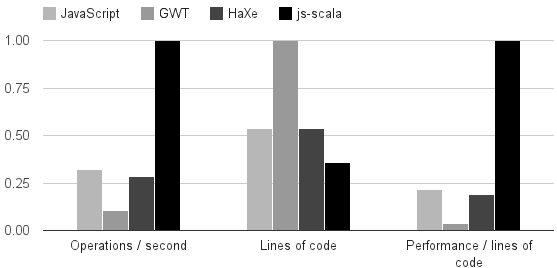
\includegraphics[width=8cm]{microbenchmark.png}
\caption{Micro-benchmark on the optional values abstraction}
\label{micro-benchmark}
\end{figure}

Figure \ref{micro-benchmark} shows the micro-benchmark results. Js-scala is between 3 to 100 times
faster than other approaches on our benchmark. Combined with the fact that it provides high-level
abstractions, it has a performance / lines of code ratio more than 4 times higher than other
approaches.

\subsection{Real World Application}

Chooze~\footnote{\href{http://chooze.herokuapp.com}{http://chooze.herokuapp.com}} is an existing
complete application for making polls. It allows users to create a poll, define the choice
alternatives, share the poll, vote and look at the results. It contains JavaScript code to handle
the dynamic behavior of the application: double-posting prevention, dynamic form update and rich
interaction with the document.

The application was initially written using jQuery. We rewrote it using several technologies for the
client-side part: vanilla JavaScript (low-level code without third-party library), js-scala, GWT and
HaXe. In each case we tried to write the application in an idiomatic way\footnote{Source code is
available at \href{http://github.com/julienrf/chooze}{http://github.com/julienrf/chooze}}.

\subsubsection{Performance}

The benchmark code simulates user actions on a Web page (2000 clicks on buttons, triggering a
dynamic update of the page and involving the use of the optional value monad, the selectors API and
the HTML fragment definition API). Figure \ref{benchmark} shows the benchmark results.

\begin{figure}
\centering
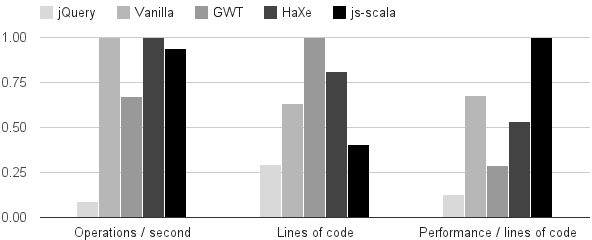
\includegraphics[width=8cm]{chooze.png}
\caption{Benchmarks on a real application}
\label{benchmark}
\end{figure}

The runtime performances of the vanilla JavaScript, HaXe and js-scala versions are similar (though
the js-scala version is slightly slower by 6\%). It is worth noting that the vanilla JavaScript and
the HaXe versions use low-level code compared to js-scala, as shown in the second part of the figure
(lines of code): the js-scala version needs only 74 lines of code while the vanilla JavaScript
version needs 116 lines of code (57\% bigger) and the HaXe version needs 148 lines of code (100\%
bigger). The jQuery JavaScript version, of which code is high-level (54 lines of code, 27\% less
than js-scala) runs 10 times slower than the js-scala version.

The last part of the figure compares the runtime performance / lines of code ratio. Js-scala shows
the best score, being 1.48 times better than the vanilla JavaScript version, 1.88 times better than
the HaXe version, 3.45 times better than the GWT version and 7.82 times better than the jQuery
JavaScript version.

\subsubsection{Code Reuse}

We were able to share HTML DOM fragment definitions between server-side and client-side in js-scala.

\section{Conclusion}
\label{discussion}

We implemented a high-level language abstracting over client and server heterogeneity but producing
efficient code.
Generated code size?

%\appendix
%\section{Appendix Title}
%
%This is the text of the appendix, if you need one.
%
\acks

This work was funded by Zenexity.

\bibliographystyle{abbrvnat}
\bibliography{biblio}
%\begin{thebibliography}{}
%\softraggedright
%
%\bibitem[Smith et~al.(2009)Smith, Jones]{smith02}
%P. Q. Smith, and X. Y. Jones. ...reference text...
%
%\end{thebibliography}
%
\end{document}
